% Topic 6: Simultaneous Linear Equations with More Than Two Variables
% Part of the Matrix Fundamentals section

\subsection{Simultaneous Linear Equations with More Than Two Variables}

When we move from two variables ($x, y$) to three variables ($x, y, z$), the geometric interpretation expands from two-dimensional space to three-dimensional space.

A linear equation in two variables ($ax + by = c$) represents a \textbf{line}. \\
A linear equation in three variables ($ax + by + cz = d$) represents a \textbf{flat plane} in 3D space.

\subsubsection*{Geometric Interpretations in 3D}

When solving a system of three linear equations in three variables, we are looking for the point(s) in 3D space where all three planes intersect. There are three main categories of outcomes:

\begin{itemize}[leftmargin=*]
  \item \textbf{Unique Solution:} The three planes meet at a single, distinct point.
  \item \textbf{Infinitely Many Solutions:} The planes intersect along a common line (like the pages of a book meeting at the spine), or all three equations represent the exact same plane.
  \item \textbf{No Solution:} There is no single point that belongs to all three planes. For example, two planes might be parallel, or they might form a triangular prism (like a tent) where they intersect in pairs but never all three together.
\end{itemize}

\begin{center}
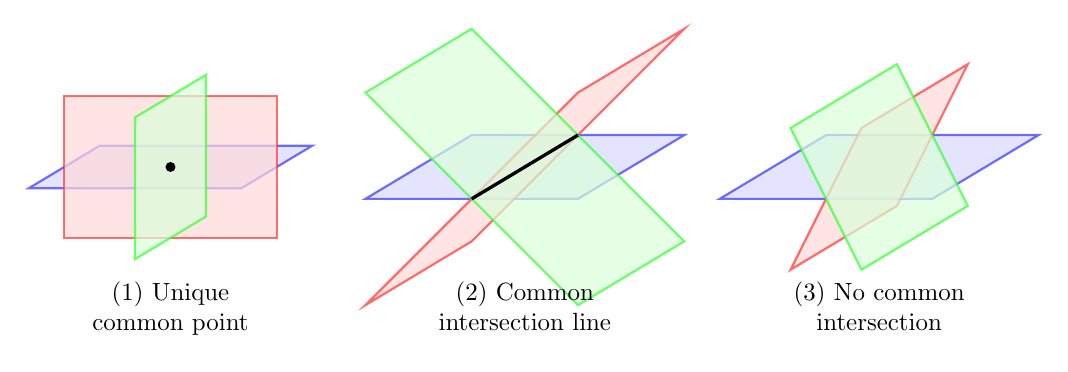
\begin{tikzpicture}[scale=0.9, every node/.style={scale=0.9}]
  % 1) Unique point
  \begin{scope}[shift={(0,0)}]
    \filldraw[fill=blue!15, draw=blue!80, thick, opacity=0.7] (1.00,-0.30) -- (2.00,0.30) -- (-1.00,0.30) -- (-2.00,-0.30) -- cycle;
    \filldraw[fill=red!15, draw=red!80, thick, opacity=0.7] (1.50,1.00) -- (-1.50,1.00) -- (-1.50,-1.00) -- (1.50,-1.00) -- cycle;
    \filldraw[fill=green!15, draw=green!80, thick, opacity=0.7] (-0.50,0.70) -- (0.50,1.30) -- (0.50,-0.70) -- (-0.50,-1.30) -- cycle;
    \fill[black] (0,0) circle (2pt);
    \node[align=center, below] at (0,-1.5) {(1) Unique\\common point};
  \end{scope}

  % 2) Common line
  \begin{scope}[shift={(5,0)}]
    \filldraw[fill=blue!15, draw=blue!80, thick, opacity=0.7] (0.75,-0.45) -- (2.25,0.45) -- (-0.75,0.45) -- (-2.25,-0.45) -- cycle;
    \filldraw[fill=red!15, draw=red!80, thick, opacity=0.7] (0.75,1.05) -- (2.25,1.95) -- (-0.75,-1.05) -- (-2.25,-1.95) -- cycle;
    \filldraw[fill=green!15, draw=green!80, thick, opacity=0.7] (0.75,-1.95) -- (2.25,-1.05) -- (-0.75,1.95) -- (-2.25,1.05) -- cycle;
    \draw[black, very thick] (0.75, 0.45) -- (-0.75, -0.45);
    \node[align=center, below] at (0,-1.5) {(2) Common\\intersection line};
  \end{scope}

  % 3) Prism (no common intersection)
  \begin{scope}[shift={(10,0)}]
    \filldraw[fill=blue!15, draw=blue!80, thick, opacity=0.7] (0.75,-0.45) -- (2.25,0.45) -- (-0.75,0.45) -- (-2.25,-0.45) -- cycle;
    \filldraw[fill=red!15, draw=red!80, thick, opacity=0.7] (-0.25,0.55) -- (1.25,1.45) -- (0.25,-0.55) -- (-1.25,-1.45) -- cycle;
    \filldraw[fill=green!15, draw=green!80, thick, opacity=0.7] (-1.25,0.55) -- (0.25,1.45) -- (1.25,-0.55) -- (-0.25,-1.45) -- cycle;
    \node[align=center, below] at (0,-1.5) {(3) No common\\intersection};
  \end{scope}
\end{tikzpicture}
\end{center}

\subsubsection*{Setting Up Systems}

To find a unique solution for $n$ unknown variables, you generally need $n$ independent linear equations. A common application is translating real-world scenarios into a $3 \times 3$ system of equations.

\bigskip

% ── Worked Example: Setting up a 3x3 system ──
\begin{problem}[Translating a Word Problem into a System]
A local bakery sells three types of cakes: chocolate, vanilla, and strawberry. The bakery records its sales and revenue for three consecutive days:
\begin{itemize}
  \item \textbf{Monday:} 2 chocolate, 3 vanilla, and 1 strawberry cake were sold for a total of \$115.
  \item \textbf{Tuesday:} 1 chocolate, 2 vanilla, and 2 strawberry cakes were sold for a total of \$110.
  \item \textbf{Wednesday:} 3 chocolate, 1 vanilla, and 3 strawberry cakes were sold for a total of \$165.
\end{itemize}

Assuming the price of each cake type remains constant, define appropriate variables and set up a system of three simultaneous linear equations that models this situation.
\end{problem}

\begin{solution}
\textbf{Step 1: Define the variables.} \\
Let $x$ = the price of a chocolate cake (in \$). \\
Let $y$ = the price of a vanilla cake (in \$). \\
Let $z$ = the price of a strawberry cake (in \$).

\medskip
\textbf{Step 2: Translate each day's sales into an equation.} \\
Monday's sales ($2$ choc, $3$ van, $1$ straw yield \$115):
\[ 2x + 3y + z = 115 \]
Tuesday's sales ($1$ choc, $2$ van, $2$ straw yield \$110):
\[ x + 2y + 2z = 110 \]
Wednesday's sales ($3$ choc, $1$ van, $3$ straw yield \$165):
\[ 3x + y + 3z = 165 \]

\medskip
\textbf{Step 3: State the final system.} \\
The system of simultaneous linear equations is:
\begin{align*}
2x + 3y + z &= 115 \\
x + 2y + 2z &= 110 \\
3x + y + 3z &= 165
\end{align*}

\emph{(Note: We will solve this exact system using matrices in the next topic!)}
\end{solution}

\begin{takeaways}
\item \textbf{Geometry of $3$ Variables:} Always visualize $3 \times 3$ systems as three flat planes in 3D space. When a unique solution exists, it is the common intersection point.
\item \textbf{Information Requirement:} Solving for 3 unknowns uniquely requires 3 independent pieces of information (equations). If you only have two equations, two independent consistent planes normally intersect in a line; parallel planes have no common points and coincident planes give a plane of solutions.
\item \textbf{Careful Translation:} When reading word problems, ensure the coefficients (quantities) align correctly with their corresponding variables (prices) in each equation.
\end{takeaways}
